% - MTSA
%     Herramienta, sintaxis
% - Tests 
%     Qué tests desarrollamos, quizás mostrar un par interesantes y explicarlos

El algoritmo fue implementado en el lenguaje Java, agregando a la funcionalidad del programa Modal Transition System Analyser (MTSA)\cite{mtsaRepo}.

\section{MTSA}
El software utilizado cuenta con una gran cantidad de funcionalidad. Principalmente nos interesa la forma de escribir Labelled Transition Systems (LTS), esto se puede hacer mediante Finite State Process (FSP). En el listing~\ref{ejLTS} volvemos al caso de estudio presentado en~\ref{chpt:casoAviones} esta vez escrito en la herrmienta MTSA.

En primer lugar definimos las constantes que determinan la cantidad de sub-servicios a contratar. Luego definimos la componente \texttt{Agencia}, con un único estado que vuelve a sí mismo con las siguientes transiciones: \texttt{cancelacion, compra, query[servicio]}, este último se lee como cualquier transición \texttt{query[i]} si $i \in Servicio$.

Con la definición de los sub-servicios se puede ver una definición genérica compacta de múltiples componentes idénticas del problema, tantas como elementos haya en \texttt{Servicio}, cada una con su \texttt{id}, comenzado en 0, que es utilizado para definir transiciones únicas para cada componente. También se ve que para un componente más complejo simplemente se declaran más estados, cada uno con su nombre en mayúscula, sin necesidad de aclarar que pertenecen a un componente. Si se quiere que un estado tenga 2 transiciones que lleven a estados distintos se logra con el operador \texttt{|} (como ejemplo, ver el estado \texttt{Queried}).

Finalmente mostramos cómo se pueden componer las distintas LTSs con el comando \texttt{||}, con el cual nuestra planta compuesta tendrá tanto a la agencia como a los subservicios.

\begin{lstlisting}[language = mtsa, caption=Ejemplo de LTS y composición, label=ejLTS]
const N = 1
range Servicio = 0..(N-1)

Agencia = (
{cancelacion,compra} -> Agencia |
query[servicio] -> Agencia ).

SubService(id=0) = Unqueried,
Unqueried = (cancelacion -> Unqueried |
query[id] -> Queried),
Queried = (valido -> Disponible | noValido -> Imposible),
Disponible = ({compra,cancelacion} -> Unqueried),
Imposible = (canelacion -> Unqueried).

||Plant = Agencia || SubService[Servicio].
...
\end{lstlisting}

En el listing~\ref{ejController} vemos un ejemplo de cómo definir un controlador, en este caso lo llamamos $Goal$. En el área de \textit{Automated planning} el objetivo es alcanzar algún estado \textit{final}, es decir, los estados son los marcados; sin embargo en el contexto MTSA y al representar el problema con LTSs solo podemos marcar transiciones. La interpretación final es que las transiciones señaladas como \textit{marcadas} llevan a estados marcados y estos serán nuestros objetivos. En el ejemplo se declara la transición $compra$ como marcada, señalando la compra sin errores de un paquete. En este punto aclaramos, únicamente para facilitar cualquier intento de reproducción, que al utilizar transiciones marcadas, se puede generar un desdoblamiento de los estados. Como ejemplo notar que el estado \texttt{Agencia} va a tener (internamente) para la herramienta 2 versiones, una marcada alcanzada por $compra$ y otra no marcada alcanzada por $cancelacion$ y $query[servicio]$.

Luego definimos el conjunto de transiciones controlables, en este caso $cancelacion, compra$ y $ query[Servicio]$. Por último debemos agregar la palabra clave \texttt{nonblocking}, en caso contrario se intentará, por defecto, resolver otro problema de control fuera del alcance de este trabajo.

En la última línea utilizamos la palabra clave \texttt{heuristic} para aclarar que queremos utilizar el algoritmo de DCS, luego nombramos como $DirectedController$ al controlador que devuelve nuestro algoritmo cuando lo definimos como el LTS $Compuesto$ ($Plant$)\footnote{Cabe destacar que a esta altura la composición todavía no fue calculada} que cumple con la especificación $Goal$.

\begin{lstlisting}[language = mtsa, caption=Ejemplo de Controller y DCS, label=ejController]
...
controllerSpec Goal = {
marking = {compra}
controllable = {cancelacion, compra, query[Servicio]}
nonblocking
}

heuristic ||DirectedController = Plant~{Goal}.
\end{lstlisting}



\section{Heurística de debugging}
Como dijimos en el capítulo anterior, el algoritmo de DCS debe ser agnóstico a la heurística. Al comenzar nuestro trabajo en el proyecto y una vez que pudimos generar un conocimiento sobre el pseudocódigo nos percatamos de ciertos casos borde que no iban a ser bien resueltos, o esto suponíamos. Sin embargo, al correr dichos casos el resultado era correcto, esto se debía a que la heurística era muy buena y llevaba al error directamente; entonces no caía en nuestra ``trampa''.

En función de poner a prueba sólo el algoritmo de exploración desarrollamos una heurística de debugging o \textit{Dummy}. La misma ordena las transiciones a explorar alfabéticamente, dejando primero las no controlables pero no mira ninguna información sobre distancia a marcados o error. Decidimos dejar el ordenamiento de no controlables primero ya que esto no es heurístico, se sabe perfectamente qué transiciones son controlables y cuáles no.

A partir de entonces usamos los nombres de las transiciones para explorar nuestros casos de test de la forma que nos interesaba. 

\section{Suite de regresión}
A continuación mostraremos algunos resultados obtenidos a partir de nuestra batería de tests. La misma cuenta con \totalTests tests, todos casos sumamente especiales o variaciones pequeñas de los mismos que son interesantes desde un punto de vista implementativo. En el capítulo \ref{chpt:implementation} se puede encontrar más detalle sobre ellos y cómo los desarrollamos, junto con ejemplos de especificación del modelo.

Como podemos ver en la tabla \ref{tab:resultadosTest} los tests se comportan diferente según la heurística que se use, \textit{RA} o \textit{Dummy}. Exception refiere a un error implementativo que surgía en tiempo de ejecución, específicamente Concurrent Modification Exception, esto pasaba porque se modificaba a la vez que se recorría un conjunto de estados. \textit{Falsos  no controlables} son casos que deberían haber dado controlable y no fue así, la inversa para \textit{falsos controlables}.

%TODO acomodar estos parrafos mejor y agregar más explicación sobre las heurísticas

TIENE SENTIDO MOSTRAR ESTO? los tests se hicieron para cada versión particular, por eso algunos van a andar en el original y otros no. Tiene sentido ir mostrando el progreso y por qué rompían cada uno en cada versión aunque esto me parece un poco mucho. Un punto medio sería explicar el por qué de cada test y listo.

Cabe destacar que, además, fallan en distintos tests. Hay 4 tests que dieron falsos no controlables con \textit{RA} pero funcionaron correctamente con \textit{Dummy}. Por su lado \textit{Dummy} falla en 4 tests ``nuevos'' en esta categoría.

\begin{table}
	\centering
	\begin{tabular}{|l|c|c|c|}
		\hline
		& Exception & Falsos no controlables & Falsos controlables \\ \hline
		RA & 7 & 7 & - \\ \hline
		Dummy & 3 & 7 & 3 \\ 
		\hline
	\end{tabular}
	\caption{Resumen fallos del suite}
	\label{tab:resultadosTest}
\end{table}




\section{Testing}
Luego de haber mostrado la sintaxis con la cual desarrollamos nuestros tests vamos a hablar un poco de ellos y detalles sobre algunos a destacar. Si se desea ver la especificación de cada uno de los tests puede encontrarse en \href{https://bitbucket.org/lnahabedian/mtsa/src/master/maven-root/mtsa/src/test/resources/NonBlocking/}{el repositorio de MTSA}\footnote{https://bitbucket.org/lnahabedian/mtsa/src/master/maven-root/mtsa/src/test/resources/NonBlocking/}.

En total tenemos una batería de \totalTests tests. Los cuáles no fueron desarrollados uno detrás del otro sino que utilizamos una técnica llamada TDD (Test Driven Development). Al comienzo se nos fue presentado el algoritmo original y, luego de mirar en detalle tanto el pseudocódigo como la implementación, notamos algunos casos que quizás resolvería mal; fue entonces que iniciamos la batería de tests. 
Luego entramos en un ciclo donde fuimos generando versiones que corregían los casos y más tests que rompían otras partes del algoritmo. Además en ciertos puntos críticos decidimos refactorizar completamente partes amplias de la implementación, fuera de las refactorizaciones chicas al pasar los tests.

Como recordatorio resumimos los problemas encontrados en tres grandes grupos.
\begin{itemize}
 \item Falencias al encontrar errores
 \item Propagación local
 \item Falta de completitud
\end{itemize}

Es necesario entrar un poco en detalle sobre la implementación del algoritmo. Para manejar la exploración de manera ordenada contamos con una cola de estados ``open'', en ella colocamos los estados que están esperando para ser explorados. Notar que un estado puede salir y entrar de ``open'' varias veces, ya que podríamos estar explorando otra transición, pero sólo una ``cantidad de transiciones'' de veces. Muchos de los problemas intermedios fueron a la hora de reabrir estados, para que puedan seguir siendo explorados, esto se traducía en una finalización temprana de la exploración llegando a una conclusión incorrecta.

Dentro de esta batería los siguientes casos son de especial interés.
\bigskip

\textbf{Test 1} Fig \ref{fig:test1}
\begin{figure}
 \centering
 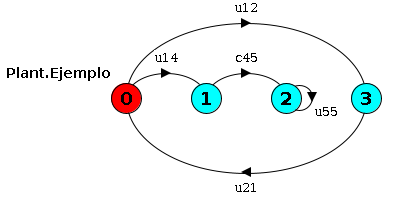
\includegraphics[scale=0.7]{figures/tests/test1.png}
 \caption{LTS del test 1}
 \label{fig:test1}
\end{figure}
Ataca el problema de falta de completitud. Luego de encontrar el primer loop no controlable (u12, u21), al ver el nodo inicial nuevamente, propaga mal lo que en la versión anterior era conocido como WEAK, es decir, sabemos que está activo pero no tenemos datos suficientes para cerrarlo. El problema es que no vuelve a poner al nodo inicial en la cola de exploración, por ende no ve el otro camino, que lleva al estado marcado (y finalmente Goal).

% \smallskip
% \textbf{Test 7} Es una suma y refinamiento de tests anteriores. La intención es ver cómo maneja distintos tipos de loops. Encontraba un loop que pensaba era Goal pero luego, recién al querer crear controloador, fallaba porque aún tenía estados por explorar. Esto era doblemente malo porque se puede tener una conclusión errónea y no se sigue explorando.
% TODO dejamos el test 7? es medio gigante y no tiene algo que otros no. Quizás mejor mostrar varios, más chicos

\smallskip
\textbf{Test 8} Fig \ref{fig:test8} Es un problema de falencias al encontrar errores ya que no señala el estado 3 como error, porque no detecta que es un livelock. Notar que esto sería lo mismo que si tenemos una rama totalmente explorada a partir de u33.
\begin{figure}
 \centering
 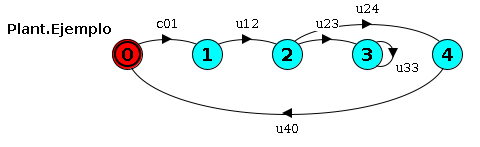
\includegraphics[scale=0.7]{figures/tests/test8.png}
 \caption{LTS del test 8}
 \label{fig:test8}
\end{figure}

TEST 12, este puede ser otro problema? porque daba no controlable, en realidad lo es pero mepa que no detectaba que podía cortar la controlable porque está marcada?

\smallskip
\textbf{Test 26?} este puede ser interesante porque son dos loops no controlables pero ganas en ambos y dice ``Caso para intentar mostrar que ver solo loops minimales no sirve''. %TODO volver a verlo en detalle y escribir la explicación, debería tener que ver con ``propagación local no sirve''

TEST 30, ACÁ ESTÁ LA PAPA. otro caso de ``propagación local no sirve''. 2 y 3 son goal, pero al querer propagar a 0 dice ``uh esta no controlable me lleva a algo de estatus desconocido'' entonces no marca nada y termina diciendo que no es controlable cuando sí. %TODO mismo que para el 26

\smallskip
\textbf{Test 35} El tema es que arma un CCC y no chequea que sea válido bien, porque ya no hay loop con marcado. Entonces el build Controller se queja y da que no hay controlador. Pero si revisaba para el otro lado había un CCC válido

%TODO agregar tests que usen debuggins abs (i.e., que tengan nombres las transiciones) Ej que puede estar muy bien: TEST 41

%TODO AGREGAR LOS TESTS QUE NOS HICIERON DAR CUENTA QUE EL PROPAGATE NO PODIA SER LOCAL Y HABIA QUE MARCAR ERRORES AL TERMINAR DE EXPLORAR ALGO

%TODO agregar los tests nuevos test 47 o 48?

\begin{lstlisting}[language = mtsa, caption=Test 1 a modo de ejemplo] 
Ejemplo = A1,
A1 = (u12 -> A2 | u14 ->A4),
A2 = (u21 -> A1),
A4 = (c45 ->A5),
A5 = (u55 -> A5).

||Plant = Ejemplo.

controllerSpec Goal = {
controllable = {c45}
marking = {u55}
nonblocking
}

heuristic ||C = Plant~{Goal}.
\end{lstlisting}
